\documentclass[12pt]{article}
\usepackage[top=1in, bottom=1in, left=.75in, right=.75in]{geometry}
\usepackage{amsmath, enumerate}
\usepackage{fancyhdr}
\usepackage{graphicx, xcolor, setspace, array}
\usepackage{txfonts}
\usepackage{multicol,coordsys,pgfplots}
\usepackage[scaled=0.86]{helvet}
\renewcommand{\emph}[1]{\textsf{\textbf{#1}}}
\usepackage{anyfontsize}
\usepackage{tikz,pgfplots}
\usetikzlibrary{calc,arrows.meta}
\pgfplotsset{compat = newest}

\parindent 0pt
\parskip 4pt
\pagestyle{fancy}
\fancyfoot[C]{\emph{\thepage}}
\fancyhead[L]{\ifnum \value{page} > 1\relax\emph{Math 316: Exam 2}\fi}
\fancyhead[R]{\ifnum \value{page} > 1\relax\emph{Spring 2025}\fi}
\headheight 12pt
\renewcommand{\headrulewidth}{0pt}
\renewcommand{\footrulewidth}{0pt}
\let\ds\displaystyle

\newcommand{\be}{\begin{enumerate}}
\newcommand{\ee}{\end{enumerate}}

\begin{document}
%% Front Page
{\emph{\fontsize{20}{20}\selectfont Spring 2025 \hfill
\hfill Math 316}}

\begin{center}
{\emph{{\fontsize{20}{20}\selectfont Exam 2}
}}
\end{center}

Solutions 

\be
%% Arabic Quad
\item (15 points) Solve the quadratic equation below using the Arabic method of completing the square. Include the algebraic steps and the accompanying figure. \text{equation:} \:\:\: $x^2+12x=10$

Solution

The area consisting of a square on side $x$ and a rectangle of dimensions $12 \text{ by } x$ are rearranged into a figure that is very close to a square. The new figure is missing only 4 corners, each of area $\left(\frac{12}{4}\right)^2=3^2.$ 
%$$x^2+12x\textcolor{red}{+ 4 \left(\frac{12}{4}\right)^2}=\left(x+2\left(\frac{12}{4}\right) \right)^2.$$
%
%Returning to the original equation, we conclude $10\textcolor{red}{+ 4 \left(\frac{12}{4}\right)^2}=\left(x+2\left(\frac{12}{4}\right) \right)^2.$ Thus,
%$$x=\sqrt{10+36}-6.$$

\begin{center}
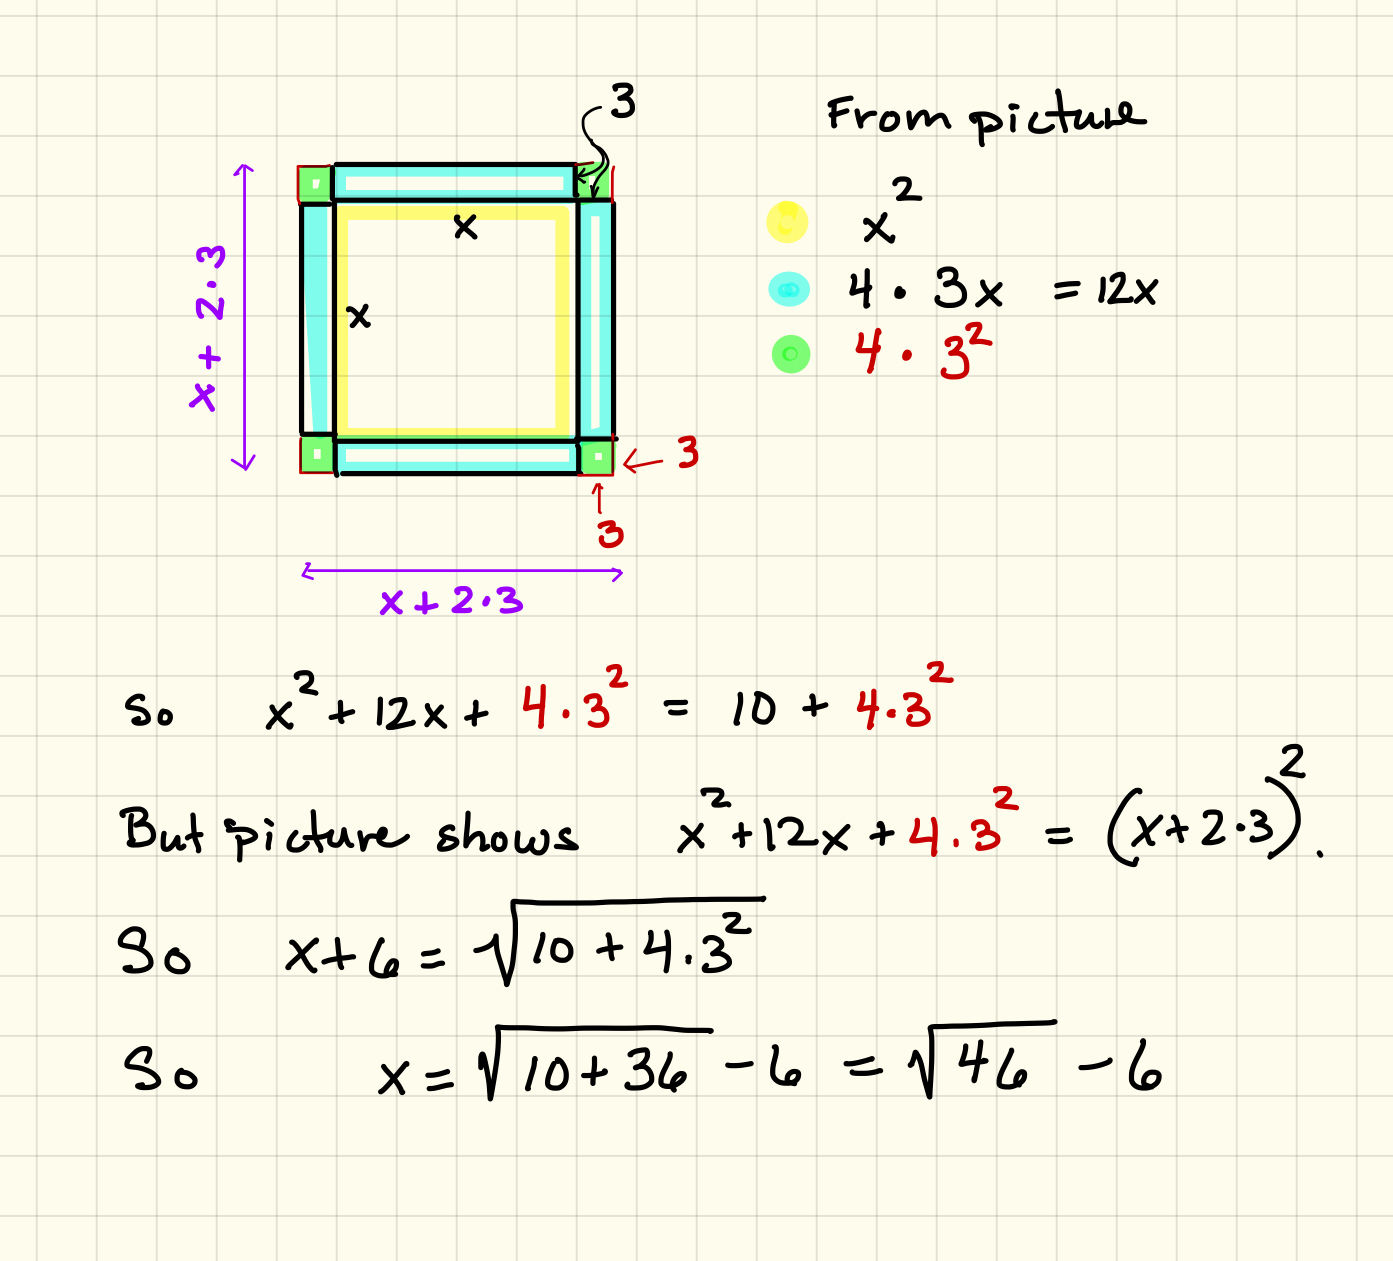
\includegraphics[scale=0.3]{e2-pic1}
\end{center}

\vfill
\textbf{Extra Credit (2 points):} Describe two ways in which the solution above is different from the modern method of completing the square.\\
\begin{itemize}
\item Only the positive square root is considered.
\item In the equation $x^2+bx$, we complete the square by adding $\left(\frac{b}{2}\right)^2$ not $4\left(\frac{b}{4}\right)^2.$
\item We think of the process in strictly algebraic terms. The square being completed is an algebraic square. No picture or physical square is present - on paper or in mind.
\end{itemize}
%%Khayyam
\item (15 points) Describe Omar Khayyam's contributions to algebra, approximately when this occurred, how his approach is similar and different from our modern approach.
	\be
	\item approximate date: 1050-1130
	\vfill
	\item description of contributions: 
	
	He showed how to find at least one positive solution to every cubic equation.
	\vfill
	\item similar to a modern approach: 
	
	He was systematic. He gave explanations of why his method worked. He realized that all cubic equations will have a solution. His amalgamation of algebra and geometry is exactly how we think about cubic equations today.
	\vfill
	\item different from a modern approach: His solutions were not numerical but graphical. That is, he described how to construct a line segment whose length was the solution. His solutions depended on understanding the conics of Apollonius, something rarely taught now. Because he needed all his coefficients to be positive and didn't want to have an equation with zero on one side of the equality, he had to consider 14 different cubic equations where we think of there only being one form of a cubic polynomial. He was limited to only considering positive roots.
	\vfill
	\ee
%%Reduced cubic
\item (20 points) 
	\be
	\item Explain what is meant by a \emph{reduced cubic}.\\
	A reduced cubic is a cubic equation for which the coefficient of the $x^2$-term is zero. One could describe it as a cubic equation with no $x^2$-term.
	
	\item Find the reduced cubic for $x^3+6x^2+x=1.$ \\
	We make a change of variable: $x=y-2.$ Then, 
	
	\begin{equation} 
	\begin{split}
	x^3+6x^2+x & = (y-2)^3+6(y-2)^2+(y-2)\\
	& = y^3-6y^2+12y-8+6y^2-24y+24+y-2\\
	&=y^3-11y+14.
	\end{split}
	\end{equation}
	
	So $x^3+6x^2+x=1$ becomes $y^3-11y+14=1$ or $y^3+13=11y.$
	\vfill
	\item What was the importance of the reduced cubic to Girolamo Cardan? 
	
	The fact that any cubic equation could be written in a reduced form meant that instead of finding algebraic formulas for all 14 different forms of the cubic, as Khayyam did, he only needed to find formulas for three of them, namely,
	$$x^3+ax=b, \: x^3 +b = ax, \: \text{and } x^3=ax+b.$$
	\vfill
	\item Describe two ways in which the Cardan's formulas for solving cubic equations catalyzed further mathematical research. Include names, dates and mathematical topic/result.
	
	Immediately after Cardan's solutions to all cubics, Ludovico Ferrari (1522-1565) produced algebraic formulas for solutions to all quartic equations which was included in \textit{Ars Magna} published in 1545. The nature of Cardan's solutions meant inevitably encountering square roots of negative numbers even when all solutions were real numbers. Thus, mathematicians began thinking about how to manipulate these structures in sensible ways. In particular, in 1572 Raphael Bombelli publishes a text describing the beginning of complex numbers.
	\vfill
	\ee
%%% 4-lines and descartes
\item (20 points)
	\be
	\item Find the locus of points, $P(x,y),$ satisfying the four line problem where the lines are
	$$L_1: x=0,\: L_2: y=0,\: L_3: x=5,\: L_4: y=10,$$
	$d_i$ is the distance between $P$ and $L_i$, and the constraint is $d_1d_2=d_3d_4.$
	
\begin{center}
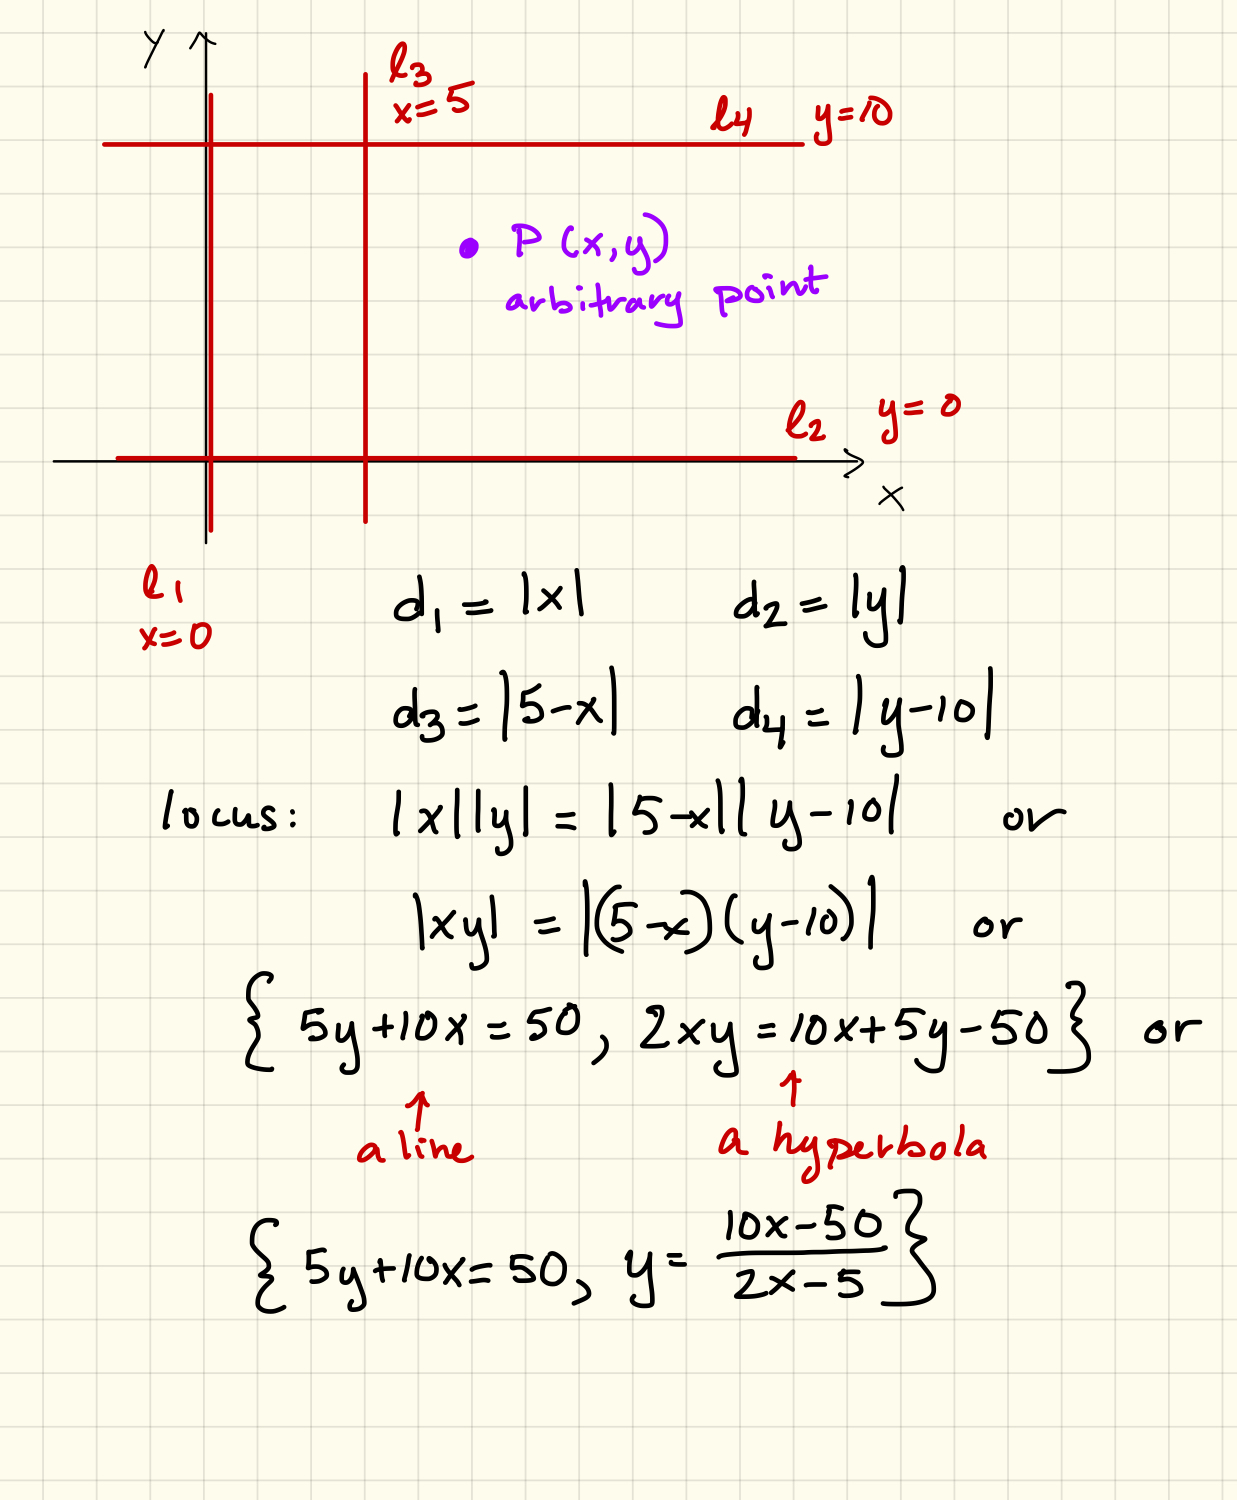
\includegraphics[scale=0.2]{e2-pic2}
\end{center}	
	
	\vfill
	\item Find two specific points in the locus.\\
	The easiest are $(0,10)$ and $(5,0)$.
	\vspace{0.5in}
	\item These ``$n$ line problems" (4 line problem, 5 line problem, etc) appear in Ren\'{e} Descartes' La G\'{e}om\'{e}trie. Why? What was Descartes attempting to demonstrate?\\
	
	La G\'{e}om\'{e}trie was an appendix to a treatise on systematic ways of approaching problems in mathematics and science. The idea is to be excruciatingly careful about determining what you know. This was supposed to be an illustration of the method in action.
	
	More specifically, the Four-Line Problem had already been proposed and solved by Pappus but without proof. Moreover, Pappus had no solutions for the Five-Line Problem or the $n$-line problem for any integer $n$ larger than 4. Thus, Descartes' solutions demonstrated the power of his approach -- both philosophical and mathematical -- by providing proof that Pappus' assertion was correct and demonstrating solutions to problems that Pappus could not solve. 
	
		\vfill
	\item \textbf{extra credit (2 points)} Describe in words or by a graph what the locus of points from part (a).\\
	The locus consists of the line $y=10-2x$ and the rational function $y=\frac{10x-50}{2x-5}$. They are both easy to draw.
	\ee
%%calculus
\item (15 points) Give an example of a mathematician who solved a problem we could consider a typical calculus 1 problem prior to 1700. Describe their approach and compare it to our modern approach to the problem.
	\be
	\item Name of mathematician and approximate dates: John Wallis, 1655, in \textit{Arithmetica Infinitorum}
	\vfill
	\item Description of calculus problem: Find the area under the curve $y=x^k$  from $x=0$ to $x=a$ for positive integers $k=2,3,4...$
	\vfill
	\item Their method/strategy of solution: Approximate the ratio of the area under the curve to the area of the circumscribing rectangle using Riemann-sum-style rectangles.
	\vfill
	\item Similarities: He seems to be imagining the same sort of rectangles that we learn in Calculus I  where the bases have progressively smaller width and then uses knowledge about convergent series. 
	\vfill
	\item Differences: He uses different notation such as no limit or integral sign. He does not use the Fundamental Theorem of Calculus or antiderivatives. Instead he uses formulas for sums of the form $\sum_{i=0}^n \frac{1}{n^k}$  and $\sum_{i=0}^n (k+1)^k$ for various integers $k.$ His final answer is not actually the area under the curve, but the ratio of the area under $y=x^k$ on $[0,a]$ to the area of the rectangle determined by $(0,0)$ and $(a,a^k).$ The method was limited by an understanding of infinite series, thus he could't apply it to, say, function with fractional exponents.
	\vfill
	\ee
\item (15 points) List five significant mathematical contributions of Isaac Newton and/or Gottfried Leibniz. Indicate which of the two discovered/developed the concept. Make sure you include \textbf{at least one contribution from each person}.
	\be
	\item[(1):] Newton and Leibniz: The Fundamental Theorem of Calculus. That is, if the expression, $D,$ is obtained when finding the slope of a curve $C$, the expression $C$ is used to find the area under the curve $D.$ \\
	
	\vfill
	\item[(2):] Newton: The generalized Binomial Theorem. \\

	\vfill
	\item[(3):] Leibniz: The derivative rules we learn in Calculus I including rules about sums, differences, products and quotients. \\

	
	\item[(4):] Newton: A systematic approach to what we now call implicit differentiation. \\

	\vfill
	\item[(5):] Leibniz: Intuitive notation such has differentials and integral signs to represent small changes or infinite sums respectively.\\

	\vfill
	\ee
	
\ee


\end{document}

%%%%ENDDOCUMENT


